In the last chapter we described the mathematical background behind reinforcement learning and how a problem can be modeled with it.
We also saw that for problems with continuous state and/or action spaces, it can be necessary to use function approximators such as
neural networks. 
In this chapter we  will describe the theoretical background of NNs, as function approximators.

Deep learning is a field of Machine Learning that in part studies deep neural networks and how they learn. 

\section{History}
Today, Deep learning is a very significant topic for the scientific community yet its history goes back since the 1940s \cite{DeepLearningBook}.

There has been a major resurgence of deep learning mainly because computers today became faster.
Training large deep learning models are computationally very expensive and could be sped up with the use
of graphics processing units (GPUs).

Artificial Neural Networks are one of the earliest learning algorithms. The novel concept behind it was to 
create mathematical models that tried to mimic the brain.
NNs were based on the human brain's neurological structure, more specifically neurons and how they connect with other neurons.
Figure \ref{fig:neuron} illustrates a single neuron cell.

\begin{figure}
    \centering
    \includegraphics[width=1\textwidth]{Chapter3/neuron.png}
    \caption{Neuron unit cell structure.}
    \label{fig:neuron}
\end{figure}

A neuron cell is capable of transmitting information by sending electrical and chemical signals through axons and they connect to other neurons
forming neural networks. The human brain, for example, has billions of connected neurons.
NNs, therefore, are a simplified mathematical representation of neurons: essentially, a neuron can be viewed as a cell that receives one or more inputs
and produces one or more outputs.

\section{Neural Networks}

\subsection{Representation}
\label{sec:rep}

In simple terms, a neural network is a mathematical structure that receives an input and calculates an output.
We will describe a simple NN known as feedforward neural network or Multi Layer Perceptron (MLP).

A neural network is composed of multiple layers where each layer has one or more nodes (neurons).
The NN receives an input and computes the output according to the network architecture and parameters $\theta$.
Each input, called sample or example, is a n-dimensional feature vector $x$, and is represented as a column vector:

\begin{equation}
    x = \begin{bmatrix}
            x_1 & x_2 & x_3 & x_4 & \dots & x_{n-1} & x_{n}
        \end{bmatrix}^\intercal
\end{equation}

$x$ is known as the input layer, and each coordinate represents each of the sample's features.
The output is a k-dimensional vector $y$, known as the output layer. 
Every other layer that is not the input nor the output layer is known as a hidden layer.

In this work, note that every time we refer to an element $z^{[l]}$ we are referring to an element of the $l$-th layer.

Figure \ref{fig:neuralnet} illustrates a very simple NN with a 3-dimensional feature vector, 1-dimensional output vector and only one hidden layer.

\begin{figure}[ht]
    \centering
    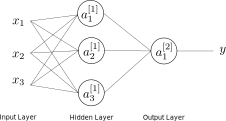
\includegraphics[width=0.75\textwidth]{Chapter3/neuralnet.pdf}
    \caption{Simple neural network.}
    \label{fig:neuralnet}
\end{figure}

Every node of the network is computed using the values from the previous layer. 
For the MLP, the node computation model is done through
a linear model $f(x; \theta)$, with $\theta$ consisting of internal parameters $w$ (weights) and $b$ (bias).
$w$ has the same dimensions as the input and $b$ is a scalar.
In this work, we treat $w$ as a column vector.

\begin{equation}
    w = \begin{bmatrix}
            w_1 & w_2 & w_3 & w_4 & \dots & w_{n-1} & w_{n}
        \end{bmatrix}^\intercal
\end{equation}

The model is defined as

\begin{equation}
    z = w^Tx + b
\end{equation}

The output of the node $a$, also known as the activation, is calculated with $x$, $b$ and 
a function $\sigma : \mathbb{R} \rightarrow \mathbb{R}$:

\begin{equation}
    a = \sigma(z) = \sigma(w^T x + b) = \sigma \bigg(\sum_{i=1}^n w_i x_i + b \bigg)
\end{equation}

Figure \ref{fig:neuralnet_out} illustrates the output of a single neuron.

\begin{figure}[ht]
    \centering
    \includegraphics[width=0.6\textwidth]{Chapter3/neuralnet_output.png}
    \caption{Node computation.}
    \label{fig:neuralnet_out}
\end{figure}

$\sigma$ is called activation function, applied to the model output ($z$).
The activation function normally is a non-linear function and its most used common choice
today is the \textbf{rectified linear unit} \cite{ReLU} or ReLU
and is defined as $\sigma(z) = max\{z, 0\}$, shown in \ref{fig:relu}. 

\begin{figure}[h]
    \centering
    \includegraphics[width=0.75\textwidth]{Chapter3/relu.pdf}
    \caption{Linear rectified unit plot.}
    \label{fig:relu}
\end{figure}

Other examples of popular activation functions are $\sigma(z) = \frac{1}{1 + e^{-z}}$, known as the sigmoid function
and $tanh(z)$ \cite{ActivationFunction}.

A neural network is therefore is a connection of multiple neurons as inputs to other neurons.
Let us return our attention to the network from Figure \ref{fig:neuralnet}.
We denote $(W,b) = (W^{[1]}, b^{[1]}, W^{[2]}, b^{[2]})$ as the network parameters, where $W^{[l]}$ is 
the matrix formed by concatenating the individual parameters of the $l$-th layer such that
$W_{ij}$ denotes the parameter associated with the connection between neuron $j$ from the $l$-th layer 
and neuron $i$ from layer $l + 1$.
Similarly, $b^{[l]}$ is the concatenation of the biases $b$ of each neuron of layer $l + 1$ and 
$b_i^{[l]}$ the bias of the $i$-th neuron of layer $l + 1$.

For the network depicted in Figure \ref{fig:neuralnet}, we are now capable of calculating the output $y$.

For the first layer: 

\begin{equation}
    z^{[1]}  = W^{[1]}x + b^{[1]} 
\end{equation}

\begin{equation}
   a^{[1]}  = \sigma(z^{[1]})
\end{equation}

And for the second layer:

\begin{equation}
    z^{[2]} = W^{[2]}a^{[1]} + b^{[2]}
\end{equation}

\begin{equation}
    y = a^{[2]} = \sigma(z^{[2]})
\end{equation}

We can think of the neural network as a recursive structure where each activation is calculated with the past's layers activation.
$a^{[l]}$ can be computed as:

\begin{equation}
    z^{[l]} = W^{[l]}a^{[l-1]} + b^{[l]}
    \label{eq:nn}
\end{equation}

\begin{equation}
    a^{[l]} = \sigma(z^{[l]})
\end{equation}

Note also that $a^{[1]} = x$.

\subsection{Vectorization}

In the previous section, we focused on computing the output of the neural network given a single sample $x$.
In modern days, however,  we are normally interested in calculating the output of a neural network for thousands or even millions of samples.

For $m$ samples, we could naively compute the output of the neural network for each example $x^{(i)}$ with Algorithm \ref{algo:naive_sample_algo}.

\begin{algorithm}[H]
    \DontPrintSemicolon
    \SetAlgoLined
    \KwResult{Output of NN for m samples.}
    \For{i = 1 to m}{
       $a^{[0]} = x^{(i)}$\;
        \For{j = 1 to L}{
            $z^{[j](i)} = W^{[j]}a^{[j-1](i)} + b^{[j]}$\;
            $a^{[j](i)} = \sigma(z^{[j](i)})$\;
        }
        $y^{(i)} = a^{[l](i)}$\;
    }
    \caption{Naive algorithm for computing NN output of $m$ samples.}
    \label{algo:naive_sample_algo}
\end{algorithm}

In practice this algorithm runs relatively slow since it computes the output of the network sequentially for each sample and 
we will apply vectorization to achieve a much faster algorithm.

Firstly, Vectorization is a technique that transforms a set of computations done sequentially in a for loop into matrix operations.
We will now vectorize our initial problem.

Let us define the following matrices

\begin{itemize}
    \item $X$ is a matrix where column i is the i-th sample $x^{(i)}$ and $W^{[l]}$. 
    We can analogously define matrices A and Z.
        $ X = \begin{bmatrix}
        x^{(1)} & x^{(2)} &  \dots  & x^{(m)} 
        \end{bmatrix}$.

    \item $W^{[l]}$ is the  weight matrix for the $l$-layer, as defined in Section \ref{sec:rep}. 
        % $ W^{[l]} = \begin{bmatrix}
        % \left(w^{[1]})\right)^T \\ \left(w^{[2]})\right)^T \\  \vdots  \\\left(w^{[l]})\right)^T} 
        % \end{bmatrix}$.
    \item $b^{[l]}$ is the bias vector for layer $l$, as defined in Section \ref{sec:rep}.
        % $ B^{[l]} = \begin{bmatrix}
        % b^{[1]} \\ b^{[2]} \\  \vdots \\ b^{[l]}
        % \end{bmatrix}$.
\end{itemize}

For the vectorized version of Algorithm \ref{algo:vectorized_sample}.

\begin{algorithm}[H]
    \DontPrintSemicolon
    \SetAlgoLined
    \KwResult{Output of NN for m samples.}
    \For{j = 1 to L}{
        $Z^{[j]} = W^{[j]}A^{[j-1]} + b^{[j]}$\;
        $A^{[j]} = \sigma(Z^{[j]})$\;
    }
    \caption{Vectorized algorithm for computing NN output of $m$ samples.}
    \label{algo:vectorized_sample}
\end{algorithm}

The vectorized version is much better since these matrices operations can be greatly sped up
on GPUs or hardware that have support for Streaming SIMD Extensions (SSE). The great majority of 
popular deep learning libraries use as much vectorization as they can.

\subsection{Deep Neural Networks}

We can extend the architecture we saw on Section \ref{sec:rep} to a higher number of layers called
deep neural networks. Figure \ref{fig:deepnn} illustrates a neural network with multiple hidden layers.

\begin{figure}[h]
    \centering
    \includegraphics[width=1\textwidth]{Chapter3/deep_neural_net.png}
    \caption{Neural network with multiple layer.}
    \label{fig:deepnn}
\end{figure}

The activation of layer $l + 1, l > 1$, can be calculated according to Equation \ref{eq:nn}.

\section{Learning}

As described in the previous section, feedforward networks defines a mapping $y = f(x; \theta)$,
or, equivalently, serve as general function approximators.

This section describes deep learning algorithms that learn the value of the parameters $\theta$ that best approximates $f$.

Most deep learning algorithms need to describe a cost function and optimization algorithm.

\subsection{Cost Function}

The cost function $J(\theta)$ is a metric of how good our estimator is to our dataset: the lower the cost function, the less error
the model has when predicting $y$. It describes the function that we wish to minimize and normally it envolves an average of the errors
between the the target value of a sample and the predicted value of the estimator for the sample.

For example, for the problem of linear regression where $X$ are the sample values and $y$ are the target
values for our dataset, we wish to learn the parameters $\theta$ from our function approximator $f$. 
The most used cost function for this problem is

\begin{equation}
    J(\theta) = \dfrac{1}{m} \sum_{i = 1}^m (y_i - f(x_i, \theta))^2
\end{equation}

Another example is the logistic regression problem. The most common cost function for this problem is

\begin{equation}
    J(\theta) = - \dfrac{1}{m} \sum_{i = 1}^m [y_i\log{f(x_i, \theta} + (1 - y_i)\log{1 - f(x_i, \theta)}]
\end{equation}

Choosing a good cost function greatly impacts how good the design of the deep neural network is.

% TODO Regularization

\subsection{Optimization Algorithms}

After defining a cost function, finding the parameters that effectively minimize the cost function is not trivial.
The non linearity of NN causes most cost functions to be non-convex and therefore, neural networks are usually
trained by iterative, gradient-based optimizers. In practice, however, this is very unlikely
 \cite{swirszcz2017local, goodfellow2014qualitatively, lin2017does}.

Section \ref{subsec:back_prop} describes how neural networks gradients can be calculated.

\subsubsection{Gradient Descent}

One of the most common optimization algorithm is Gradient Descent. It is an iterative first-order method
that tries to find a local minimum for a function $f$ by moving in the negative direction of its gradient.
Specifically for neural networks, our goal is to minimize the cost function $J(\theta)$. The algorithm's update step
is Equation \eqref{eq:grad_desc} done for each $\theta_i$

\begin{equation}
    \theta_i = \theta_i - \alpha \dfrac{\partial J}{\partial \theta_i}
    \label{eq:grad_desc}
\end{equation}

The learning rate, $\alpha$ measures how big the update step in the direction of the gradient will be.

For example, let $g:\mathbb{R}^2\to\mathbb{R}$ given by $g(x,y)=y \sin(x) - x\cos(y)$. Figure \ref{fig:grad_desc}
illustrates 5 steps of the gradient descent algorithm. Notice how the red circle is the starting point and after 
the last iteration, the algorithm arrives approximately at a local minimum.

\begin{figure}[ht]
    \centering
    \includegraphics[width=0.8\textwidth]{Chapter3/func_exam.pdf}
    \caption{Gradient descent on function g.}
    \label{fig:grad_desc}
\end{figure}

\subsubsection{Stochastic Gradient Descent}

Another popular algorithm is Stochastic Gradient Descent (SGD) that is a stochastic approximation of Gradient Descent.
Instead of calculating $J(\theta)$ as an average between all the samples, the gradient update step is done once per sample.
It calculates an approximation of the gradient and updates the parameters $\theta_i$ with every sample.
Algorithm \ref{algo:sgd} describes SGD

\begin{algorithm}[H]
    \DontPrintSemicolon
    \SetAlgoLined
    \KwResult{Function minimum}
    \While{An approximate minimum is not obtained} {
        Randomly shuffle examples in the training set\;
        \For{i = 1,2,..., m} {
            $\theta_i = \theta_i - \alpha \nabla J_i(\theta)$\;
        }
    }
    \caption{SGD algorithm.}
    \label{algo:sgd}
\end{algorithm}

The gradient approximation for SGD is much faster to compute, however, since it is a noisy estimate of the gradient,
SGD may need more steps to converge to a local minimum.

\subsubsection{Mini-Batch Gradient Descent}
Finally, Mini-Batch Gradient Descent combines the idea from Gradient Descent and SGD.
It computes the gradient using more than one training example, called a \textit{mini-batch}, at each step. It may result
in smoother convergence and the code can be accelerated by making use of vectorization.

\section{Back Propagation}
\label{subsec:back_prop}

We have seen how a few gradient-based optimization algorithms work. 
To minimize the cost function we need to compute the partial derivatives of the cost function w.r.t. 
to each weight of the neural network. Calculating these partial derivatives manually would be computacionally
infeasible for large networks.
In deep neural networks, by using the chain rule, we can calculate the partial derivatives in an efficient and
compact way.

Backpropagation is an algorithm that computes the gradients of the loss function w.r.t. each input from the network.

% % Gradient image

% Therefore numerical gradient computation is an important step in deep learning.
